\newpage
\clearpage
\section{Conclusões}
\label{conclusion}
As técnicas de segmentação representam uma ferramenta valiosa para a identificação de regiões de interesse em imagens, abordando desde situações mais simples, abordadas pelas técnicas de segmentação tradicionais (Capítulo \ref{segment}), até cenários mais complexos, resolvidos pela segmentação semântica (Capítulo \ref{semantic}). Este último tipo de segmentação, em particular, apresenta semelhanças com a compreensão humana de cenários \citep{Mohan2020}, uma vez que classifica cada pixel em uma cena, atribuindo-os a diversas classes. Tal capacidade só foi alcançada graças à evolução das arquiteturas de redes neurais profundas (Capítulo \ref{cnn}), que apresentam habilidades melhoradas de aprendizado e adaptação em resposta aos problemas fornecidos.

Em uma análise mais específica, focada no campo do aprendizado de imagens, as redes neurais convolucionais ganharam destaque (Capítulo \ref{cnn}). Esta evolução entre as redes neurais profundas, as convolucionais e a segmentação semântica direcionou o estudo para o teste de um método de \textit{pooling}, introduzido no contexto das CNNs, que preservasse a espacialidade das amostras, mantendo seus valores fundamentais, como explorado no Capítulo \ref{project}. O desenvolvimento desse método respondeu à primeira questão levantada nos objetivos deste trabalho, delineados na introdução (\ref{intro}).

A aplicação do método \textit{Block-based Principal Component Analysis Pooling}, ou BPCAPooling, acompanhou a evolução das redes, iniciando sua aplicação em uma arquitetura comumente utilizada para as CNNs, a VGG-16. O objetivo era coletar insumos e avaliar a sua aplicabilidade como substituto dos métodos convencionais. Os resultados e discussões desses experimentos, detalhados no Capítulo \ref{results}, revelaram que os métodos convencionais - \textit{Max Pooling} e \textit{Avg Pooling} - ainda são superiores nos dois conjuntos de dados testados em problemas de classificação de imagens.

O melhor modelo utilizando \textit{Max Pooling} alcançou uma acurácia de $46,071\%$ e uma \textit{loss} de $1,4862$, no primeiro conjunto de dados, enquanto obteve uma acurácia de $50,080\%$ e uma \textit{loss} de $2,3745$ no segundo conjunto. Já o uso do BPCAPooling resultou em apenas $17,543\%$ de acurácia e $3,5121\%$ de \textit{loss} para o primeiro conjunto, e $4,4130\%$ de acurácia e $4,4404$ de \textit{loss} para o segundo conjunto. Portanto, os resultados indicam que o método desenvolvido não é recomendado como uma alternativa viável para substituir os métodos convencionais até o momento.

Apesar dos valores de acurácia e \textit{loss} relativamente baixos, o método apresentou diferenças visuais consideráveis em relação ao método tradicional. Essas diferenças foram evidentes ao utilizar ferramentas de explicabilidade de modelos e ao examinar características das saídas das redes, conforme mencionado na Seção \ref{results:class:datasets}.

No contexto das segmentações semânticas, os resultados obtidos (Capítulo \ref{results}) revelaram comportamento diferente dos casos de classificação ao aplicar o método proposto nas arquiteturas. Os modelos U-Net com o método proposto apresentaram uma mIoU de $0,3333$, acurácia de $86,77\%$ e uma \textit{loss} de $0,6659$, enquanto o modelo com uso de \textit{Max Pooling} obteve uma mIoU de $0,3367$ e acurácia de $88,61\%$, mas com uma \textit{loss} ligeiramente superior ($0,6668$). No entanto, todos os resultados mostram diferenças mínimas tanto em métricas quanto em qualidade visual das segmentações, sugerindo o BPCAPooling como uma alternativa válida ao método convencional, não fosse pela complexidade de código agregada, o que aumenta significativamente o tempo de execução durante as fases de treinamento e validação. Entretanto, este estudo abre uma possibilidade para que métodos tradicionais de extração de atributos e manifold learning possam ser investigados como uma camada de pooling, ou ainda, uma combinação de poolings.

Portanto, para futuros desenvolvimentos, sugere-se: 1) a otimização do código desenvolvido, considerando a troca de \textit{frameworks}, visando a redução da complexidade do código; 2) testes em conjuntos de dados adicionais apropriados para a tarefa de segmentação semântica; 3) o desenvolvimento do método BPCAUnpooling para preservar a espacialidade das amostras na fase de decodificação das U-Nets; e 4) avaliar o uso da técnica BPCAPooling em outras tarefas de processamento de imagens, como para filtragem de ruído, considerando que as redes neurais profundas normalmente eliminam a camada de \textit{Max Pooling} para essa tarefa, visto que esse método acaba amplificando o ruído \citep{zhang2017beyond}. Outras sugestões são descritas a partir das Seções \ref{conclusion:class:future} e \ref{conclusion:semantic:future}.

\subsection{Trabalhos Futuros para Classificação}
\label{conclusion:class:future}
Como mencionado na Seção \ref{project:transf}, os experimentos de classificação empregaram os princípios de transferência de aprendizado, o que comumente oferece vantagens devido ao reaproveitamento de pesos de arquiteturas treinadas em grandes conjuntos de dados \citep{Pan2010}. No entanto, embora as camadas de \textit{pooling} não tenham parâmetros treináveis diretamente afetados pela retropropagação, elas influenciam diretamente as camadas de convolução subsequentes. Isso levanta a questão: \quotes{Será que o uso de transferência de aprendizado realmente contribuiu para a aplicação do método BPCAPooling nos experimentos realizados?} Uma vez que as camadas da rede passam a ficar com os pesos aquecidos, mas com o viés da utilização de um redutor de dimensionalidade que não olha para a informação espacial de um modo global, mas sim local, como é o caso do \textit{Max Pooling} e \textit{Avg Pooling}.

Além disso, outra questão pendente diz respeito a quais camadas precisam ser descongeladas para obter os melhores resultados possíveis com o método, como comentado na Seção \ref{results:class:datasets}, que demonstra maior progresso no quarto bloco convolucional.

Por fim, a complexidade do método proposto é uma limitação. Um teste realizado com a arquitetura EfficientNetB0 \citep{Tan2019Efficientnet:Networks}, que possui $17$ camadas de \textit{pooling}, substituindo os métodos convencionais por BPCAPooling resultou em um tempo estimado de treinamento da fase de aquecimento de aproximadamente \textit{2.100} horas, de acordo com os padrões de desempenho comentados na Seção \ref{results:class}.

Para futuros trabalhos que visam aplicar o método BPCAPooling como camada de \textit{pooling} para arquiteturas de classificação, sugere-se a não utilização de transferência de aprendizado para o método, mas sim a realização de fases de treinamento e validação mais extensas, além do uso de conjuntos de dados equivalentes ao ImageNet, o que é um desafio devido às necessidades de \textit{hardware} que surgiriam. Uma sugestão adicional seria propor alternativas para otimizar a complexidade do código associado ao método BPCAPooling. Por fim, uma terceira ideia para trabalhos futuros, que também exigiria considerações sobre o \textit{hardware} necessário para os experimentos, seria a aplicação de mais épocas no descongelamento de determinados blocos convolucionais durante o processo de \textit{fine-tuning}, visando permitir a exploração mais profunda dos mapas de características e potencializar os aspectos de preservação espacial.

\subsection{Trabalhos Futuros para Segmentação Semântica}
\label{conclusion:semantic:future}
Para contribuir com o avanço deste projeto, esta seção propõe identificar pontos de melhoria e desafios encontrados para a aplicação mais ampla e aprimoramento do BPCAPooling. O objetivo é potencializar seu desempenho em relação aos métodos tradicionais, não apenas reduzindo a dimensionalidade de entradas em arquiteturas de segmentação semântica, mas também preservando a informação espacial de forma global.

Um dos grandes desafios encontrados residiu na combinação dos \textit{frameworks} Tensorflow e Keras. Dado que a abordagem proposta consistia no desenvolvimento de uma camada personalizada de \textit{pooling}, erros de desenvolvimento eram comuns, afetando significativamente o tempo de implementação e outros aspectos mencionados nesta seção. Portanto, uma proposta para futuros trabalhos seria a exploração de diferentes \textit{frameworks}, como PyTorch \citep{Paszke2017AutomaticPyTorch}. Além de potencialmente melhorar o desempenho do método, conforme discutido na Seção \ref{conclusion:class:future}.

A dificuldade enfrentada com o \textit{framework} também prejudicou a aplicação do método em mais de um conjunto de dados para a tarefa de segmentação semântica. Uma excelente proposta futura seria estender os testes para um segundo conjunto de dados, preferencialmente com múltiplos objetos de interesse em cada exemplo. Conjuntos como \textit{Cityscape} \citep{Cordts2016} e \textit{Lost and Found} \citep{Pinggera2016LostVehicles} oferecem condições ideais para avaliar as capacidades de preservação de espacialidade do BPCAPooling em cenários mais complexos.

Um dos aspectos a serem explorados em pesquisas futuras diz respeito à análise da distribuição de energia dos componentes principais em relação aos autovalores. Em outras palavras, considerando que componentes principais com valores maiores indicam maior importância, seria interessante avaliar o quanto de informação está sendo preservado. Em alguns casos, pode ser vantajoso reorganizar e subdividir a informação em múltiplos componentes, garantindo assim que a quantidade de informação preservada seja significativa e relevante para a aplicação em questão.

Além disso, iniciou-se o desenvolvimento do método BPCAUnpooling, disponível no repositório do projeto \footnote{Repositório Github do projeto - \url{https://github.com/Lucs1590/USeS-BPCA}}, mas a implementação com o \textit{framework} atual representou uma barreira. Esse método seria uma abordagem de \textit{unpooling}, contrapartida ao BPCAPooling, revertendo o processo proposto por este último, preservando também a espacialidade no processo de reconstrução realizado pelas U-Nets e similares, como ilustrado na Figura \ref{results:fig:future:0}.

\begin{figure}[H]
    \centering
    \caption{Processo de redução e reconstrução de dimensionalidade com BPCAPooling e BPCAUnpooling, respectivamente.}
    \label{results:fig:future:0}
    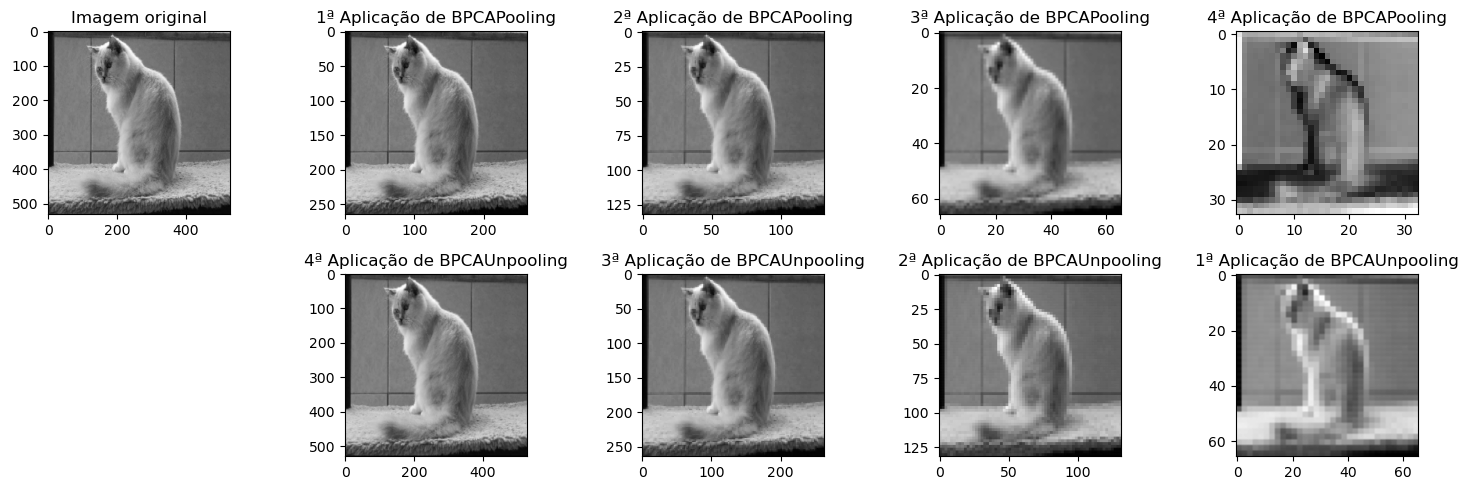
\includegraphics[width=1\textwidth]{recursos/imagens/results/bpca_unpooling.png}

    Fonte: do próprio autor.
\end{figure}

A técnica BPCAUnpooling, em contraste com o procedimento BPCAPooling, requisita a utilização de camadas densamente conectadas para obter um efeito similar ao oferecido por camadas convolucionais transpostas. A operação deste método é expressa na Equação \ref{results:eq:bpca_unpooling}, nela $\boldsymbol{X'}_{i,j,k}$ simboliza o mapa de características resultante, com suas dimensões correspondendo, respectivamente, à altura ($i$), largura ($j$) e canais ($k$).

\begin{equation}
    \label{results:eq:bpca_unpooling}
    \begin{split}
        \boldsymbol{X'}_{i,j,k} &= \text{BPCAUnpooling}(\boldsymbol{Y}_{i',j',k'}) \\
                  &= \text{reshape}\left(U \cdot \left(\text{\textit{reshape}}(S) \cdot \text{Dense}\left(\text{pad}(\boldsymbol{Y})\right)\right)\right) \cdot {\boldsymbol{\sigma}} + {\boldsymbol{\mu}}.
    \end{split}
\end{equation}

A equação expressa o processo de restauração da dimensionalidade pela aplicação do método BPCAUnpooling. Este processo envolve operações de preenchimento, remodelagem e reconstrução dos dados desagrupados com base na decomposição PCA. Na equação, o operador $\text{BPCAUnpooling}(\boldsymbol{Y}_{i',j',k'})$ retrata a execução do procedimento BPCAUnpooling ao mapa de características de entrada $\boldsymbol{Y}$.

A função $pad(\boldsymbol{Y})$ preenche o mapa de características de entrada $\boldsymbol{Y}$ com zeros, adaptando o tamanho para a subsequente atividade de \textit{unpooling}. O termo matemático $\text{Dense}(\text{pad}(\boldsymbol{Y}))$ é empregado na aprendizagem dos componentes decorrentes da PCA, por meio da camada densa com função de ativação.

A função $\text{\textit{reshape}}$ reorganiza seus argumentos para a estrutura adequada, onde $S$ simboliza os valores singulares oriundos da decomposição PCA em alinhamento com os componentes da PCA. A expressão $U \cdot (\text{\textit{reshape}}(S) \cdot \text{Dense}(\text{pad}(\boldsymbol{Y})))$ reconduz os dados desagrupados com o auxílio dos componentes e valores singulares fornecidos pela PCA.

Finalmente, a operação de multiplicação pelo desvio padrão $\boldsymbol{\sigma}$ e acréscimo da média $\boldsymbol{\mu}$ refaz a normalização inicialmente feita antes da transformação PCA.

No contexto desta equação, $U$ denota a matriz de componentes principais adquirida através da fórmula BPCAPooling, responsável por codificar a estrutura intrínseca dos dados. Esta matriz direciona a reestruturação dos dados para a dimensionalidade original.


\subsection{Considerações Finais do Capítulo}
\label{conclusion:final}
Vale citar que a partir desse trabalho foi possível submeter um artigo intitulado \textit{Exploring BPCA Pooling Layer in VGG-16 Network: A Comparative Study with Conventional Pooling Methods} na SIBGRAPI – \textit{Conference on Graphics, Patterns and Images} tendo todo o código utilizado documentado no Github \footnote{Repositório Github do trabalho da conferência - \url{https://github.com/Lucs1590/vgg_bpca}}, alvejando aumentar o nível de contribuição com a comunidade científica.

Por fim, todo o código fonte utilizado neste trabalho está documentado e disponível como \textit{open-source}\footnote{Repositório Github do projeto - \url{https://github.com/Lucs1590/USeS-BPCA}}, buscando fomentar contribuições e incentivar a comunidade científica a avançar no tema abordado, facilitando futuras pesquisas nesta área a partir de um ponto inicial avançado e com algumas dificuldades mitigadas.
